\documentclass[compress]{beamer}

\usepackage[T1]{fontenc} 
\usepackage{amsmath}
\usepackage{array}
\usepackage{color}
\usepackage{graphicx}
\usepackage[section]{placeins} % force � mettre l'image o� on veut
\usepackage{float} %utiliser H pour forcer � mettre l'image o� on veut
\usepackage{lscape} %utilisation du mode paysage
\usepackage{pslatex}
\usepackage{multimedia}

\usetheme{Frankfurt}

\setbeamertemplate{footline}{
\leavevmode%
\hbox{\hspace*{-0.06cm}
\begin{beamercolorbox}[wd=.3\paperwidth,ht=2.25ex,dp=1ex,center]{author in head/foot}%
	\usebeamerfont{author in head/foot}\insertshortauthor%~~(\insertshortinstitute)
\end{beamercolorbox}%
\begin{beamercolorbox}[wd=.5\paperwidth,ht=2.25ex,dp=1ex,center]{section in head/foot}%
	\usebeamerfont{section in head/foot}\insertshorttitle
\end{beamercolorbox}%
\begin{beamercolorbox}[wd=.2\paperwidth,ht=2.25ex,dp=1ex,right]{section in head/foot}%
	\usebeamerfont{section in head/foot}\insertshortdate{}\hspace*{2em}
	\insertframenumber{} / \inserttotalframenumber\hspace*{2ex}
\end{beamercolorbox}}%
\vskip0pt%
}

\newcommand\bn{\boldsymbol{\nabla}}
\newcommand\bo{\boldsymbol{\Omega}}
\newcommand\br{\mathbf{r}}
\newcommand\la{\left\langle}
\newcommand\ra{\right\rangle}
\newcommand\bs{\boldsymbol}
\newcommand\red{\textcolor{red}}

\renewcommand{\(}{\left(}
\renewcommand{\)}{\right)}
\renewcommand{\[}{\left[}
\renewcommand{\]}{\right]}
\beamertemplatetransparentcovered

\title{Charged particles transport}
\author{Bruno Turcksin, Jean Ragusa \& Jim Morel}\institute{Texas A\&M University, Dept. of Nuclear Engineering}
\date{}

\begin{document}

\begin{frame}
\maketitle
\end{frame}
%---------------------------------------------------------------------------------------------
\logo{\includegraphics[height=0.5cm]{../logo_Texas.jpg}}
\begin{frame}
\frametitle{Outline}
\tableofcontents[hideallsubsections]
\end{frame}
%---------------------------------------------------------------------------------------------
\section{Introduction}
\subsection{Introduction}
\begin{frame}
\frametitle{Introduction}
\begin{itemize}
\item Radiotherapy is used for cancer treatment.
\item Used Intensity Modulated Radiation Therapy (IMRT).
\item Proton therapy contains the same physics.
\end{itemize}
\begin{figure}[H]
\centering
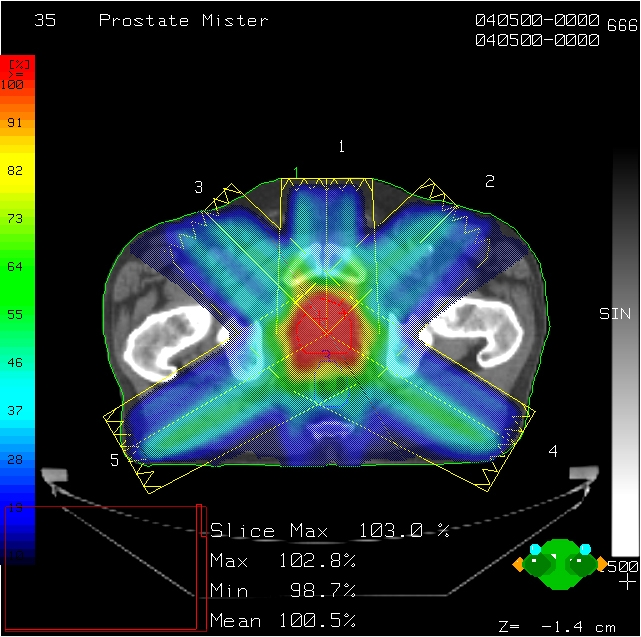
\includegraphics[width=3cm]{IMRT}
\end{figure}
\end{frame}
%---------------------------------------------------------------------------------------------
\section{Equations}
\subsection{Equations}
\begin{frame}
\frametitle{Equations}
\begin{itemize}
\item Boltzmann equation could be used but electron cross section very peaked $\rightarrow$ need very high order of Legendre polynomials ($\sim 200$) to approximate the cross section.
\item The Boltzmann-Fokker-Planck equation uses a Boltzmann scattering term for large angle scattering (hard scattering) and the Fokker-P
\end{itemize}
\end{frame}
%---------------------------------------------------------------------------------------------
\section{Optimization}
\subsection{Optimization}
\begin{frame}
\frametitle{Optimization}
\end{frame}
%---------------------------------------------------------------------------------------------
\section{Conclusions}
\subsection{Conclusions}
\begin{frame}
\frametitle{Conclusions}
\end{frame}

\end{document}
